\documentclass[a4paper, 12pt]{article}
\usepackage[utf8]{inputenc}
\usepackage[english,russian]{babel}
\usepackage[warn]{mathtext}
\usepackage{graphicx}
\usepackage{float}
\usepackage{multirow}
\restylefloat{table}
\usepackage{amsmath}
\usepackage{floatflt}
\usepackage[T2A]{fontenc}
\usepackage[left=20mm, top=20mm, right=20mm, bottom=20mm, footskip=10mm]{geometry}

\tolerance 1414
\hbadness 1414
\emergencystretch 1.5em
\hfuzz 0.3pt        % размер максимального переполнения без warning'a
\widowpenalty=10000 % запрещает одиночную строку абзаца в начале страницы
\vfuzz \hfuzz
\raggedbottom       % если на странице мало содержимого, добавить пустое место в конце, а не в середине страницы



\begin{document}

\begin{titlepage}
	\centering
	\vspace{5cm}
	{\scshape\LARGE московский физико-технический институт (национальный исследовательский университет) \par}
	\vspace{6cm}
	{\scshape\Large Лабораторная работа 1.2 \par}
	{\huge\bfseries Эффект Комптона \par}
	\vspace{1cm}
	\vfill
\begin{flushright}
	{\large Б03-104}\par
	\vspace{0.3cm}
	{\LARGE Куланов Александр}
\end{flushright}
	

	\vfill


	Долгопрудный, 2023 г.
\end{titlepage}

\begin{itemize}
	\item \textbf{Цель работы:}  с помощью сцинтилляционного спектрометра исследуется энергетический спектр $\gamma$-квантов, рассеянных на графите. Определяется энергия рассеянных $\gamma$-квантов в зависимости от угла рассеяния, а также энергия покоя частиц, на которых происходит комптоновское рассеяние.
\end{itemize}

\section{Теоретические сведения}

Рассеяние $\gamma$-лучей в веществе относится к числу явлений, в которых особенно ясно проявляется двойственная природа излучения. Волновая теория, хорошо объясняющая рассеяние длинноволнового излучения, испытывает трудности при описании рассеяния рентrеновских и $\gamma$-лучей. Эта теория, в частности, не может объяснить, почему в составе рассеянного излучения кроме исходной волны, с частотой $\omega_0$, появляется дополнительная длинноволновая компонента, отсутствующая в спектре первичного излучения.

Появление этой компоненты легко объяснимо, если считать, что $\gamma$-излучение представляет собой поток квантов (фотонов), имеющих энергию $\hbar \omega$ и импульс $p=\hbar \omega / c$. 
\begin{figure}[H]
    \centering
    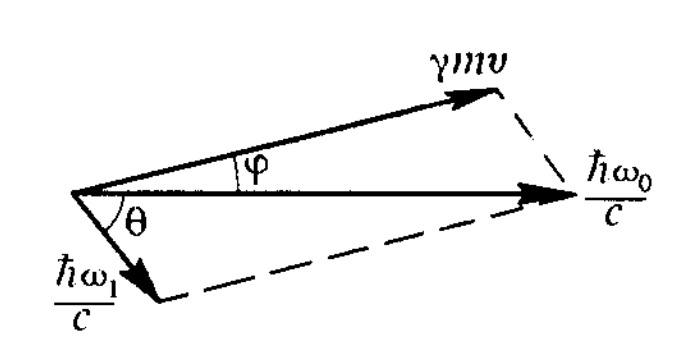
\includegraphics[width=0.5\textwidth]{diagr.jpg}
    \caption{Диаграмма рассеяния}
    \label{fig:diagr}
\end{figure}
Эффект Комптона - увеличение длины волны рассеянного излучения по сравнению с падающим - интерпретируется как результат упругого соударения двух частиц: $\gamma$-кванта (фотона) и свободного электрона.

Рассмотрим элементарную теорию эффекта Комптона. Пусть электрон до соударения покоился (еro энергия равна энергии покоя $m c^2$ ), а $\gamma$-квант имел начальную энергию $\hbar \omega_0$ и импульс $\hbar \omega_0 / c$. После соударения электрон приобретает энергию $\gamma m c^2$ и импульс $\gamma m v$, где $\gamma=\left(1-\beta^2\right)^{-1 / 2}, \beta=v / c$, а $\gamma$-квант рассеивается на некоторый угол $\theta$ по отношению к первоначальному направлению движения. Энергия и импульс $\gamma$-кванта становятся соответственно равными $\hbar \omega_1$ и $\hbar \omega_1 / c$
Запишем для рассматриваемого процесса законы сохранения энергии и импульса:
\begin{equation*}
\begin{gathered}
m c^2+\hbar \omega_0=\gamma m c^2+\hbar \omega_1, \\
\frac{\hbar \omega_0}{c}=\gamma m v \cos \varphi+\frac{\hbar \omega_1}{c} \cos \theta, \\
\gamma m v \sin \varphi=\frac{\hbar \omega_1}{c} \sin \theta .
\end{gathered}
\end{equation*}
Решая совместно эти уравнения и переходя от частот $\omega_0$ и $\omega_1 \kappa$ длинам волн $\lambda_0$ и $\lambda_1$, нетрудно получить, что изменение длины волны рассеянного излучения равно
\begin{equation}
\Delta \lambda=\lambda_1-\lambda_0=\frac{h}{m c}(1-\cos \theta)=\Lambda_K(1-\cos \theta),
\end{equation}
где $\lambda_0$ и $\lambda_1$ - длины волн $\gamma$-кванта до и после рассеяния, а величина
\begin{equation*}
\Lambda_{\mathrm{K}}=\frac{h}{m c}=2,42 \cdot 10^{-10} \mathrm{~cm}
\end{equation*}
называется комптоновской длиной волны электрона. Из формулы (1) следует, что комптоновское смещение не зависит ни от длины волны первичного излучения, ни от рода вещества, в котором наблюдается рассеяние. В приведенном выводе электрон в атоме считается свободным. Для $\gamma$-квантов с энергией в несколько десятков, а тем более сотен килоэлектрон-вольт, связь электронов в атоме, действительно, мало существенна, так как энергия их связи в легких атомах не превосходит нескольких килоэлектрон-вольт, а для большинства электронов еще меньше.

При рассеянии на связанных электронах изменение импульса кванта воспринимается атомом в целом. Поскольку масса атома очень велика, передача импульса не сопровождается сколь-нибудь заметной передачей энергии, и наблюдается несмещенная (по энергии) компонента в спектре рассеянного излучения. Таким образом, рассеяние $\gamma$-квантов на связаниых электронах можно рассматривать как упругое столкновение квантов с атомами. В классике такое рассеяние называется томсоновским и рассматривается как процесс, при котором связанные электроны атома приходят в резонансное колебание под действием падающего излучения, а затем сами излучают фотоны той же частоты. При рассеянии квантов не очень высокой энергии (единицы килоэлектрон-вольт, десятки килоэлектрон-вольт) часть электронов ведет себя, как свободные, а часть - как связанные. Оба типа рассеяния при этом наблюдаются одновременно.

Основной целью данной работы является проверка соотношения (1). Применительно к условиям нашего опыта формулу (1) следует преобразовать от длин волн к энергии $\gamma$-квантов. Как нетрудно показать, соответствующее выражение имеет вид
\begin{equation*}
\frac{1}{\varepsilon(\theta)}-\frac{1}{\varepsilon_0}=1-\cos \theta
\end{equation*}
Здесь $\varepsilon_0=E_0 /\left(m c^2\right)-$ выраженная в единицах $m c^2$ энергия $\gamma$-квантов, падающих на рассеиватель, $\varepsilon(\theta)$ - выраженная в тех же единицах энергия квантов, испытавших комптоновское рассеяние на угол $\theta, m-$ масса электрона.

Пусть $\varepsilon(\theta) = AN(\theta)$, $A$ -- коэффициент пропорциональность, $N(\theta)$ -- номер соответствующего канала. Тогда перепишем как
\begin{equation}
	\dfrac{1}{N(\theta)} - \dfrac{1}{N(0)} = A(1-\cos \theta)
\end{equation}
Отсюда можно определить энергию покоя электрона как 
\begin{equation}\label{eq:main}
mc^2 = E_\gamma \dfrac{N(90)}{N(0) - N(90)},
\end{equation}
где $E_\gamma = E_0$ -- энергия испускаемых источником $\gamma$-квантов.
\section{Экспериментальная установка}
Схема установки представлена на рисунке (\ref{fig:set})

\begin{figure}[H]
    \centering
    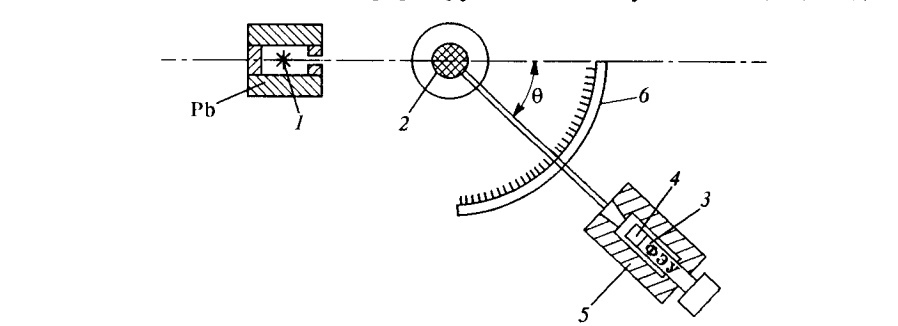
\includegraphics[width=1\textwidth]{set.jpg}
    \caption{Принципиальная схема установки}
    \label{fig:set}
\end{figure}

На Рис. изображена блок-схема установки. Источником (1) служит $^{137}Cs$, испускающий $\gamma$-лучи с энергией $662$ кэВ, который помещён в толстостенный свинцовый контейнер с коллиматором. Сформированный коллиматором узкий пучок $\gamma$-квантов попадает на графитовую мишень (2), испытывает рассеяние и регистрируется сцинтилляционным счётчиком, состоянищим из фотоэлектронного умножителя (ФЭУ) и сцинтиллятора -- выходное окно сцинтиллятора находится в оптическом контакте с фотокатодом ФЭУ. Сигналы, возникающием в аноде ФЭУ, подаются на компьютер для амплитудного анализа. Кристалл и ФЭУ расположены в светонепроницаемом блоке, укреплённого на горизонтальной штанге, которая может вместе с ним вращаться, угол поворота отсчитывается по лимбу (6). Головная часть сцинтилляционного блока закрыта свинцовым коллиматором (5), который формирует входной пучок и защищает детектор от постороннего излучения, в основном $\gamma$-квантов, проходящих через стенки защитного контейнера источника. При больших углах измерения для дополнительной защиты между контейнером и источником и детектором ставился свинцовый экран.
\begin{figure}[H]
    \centering
    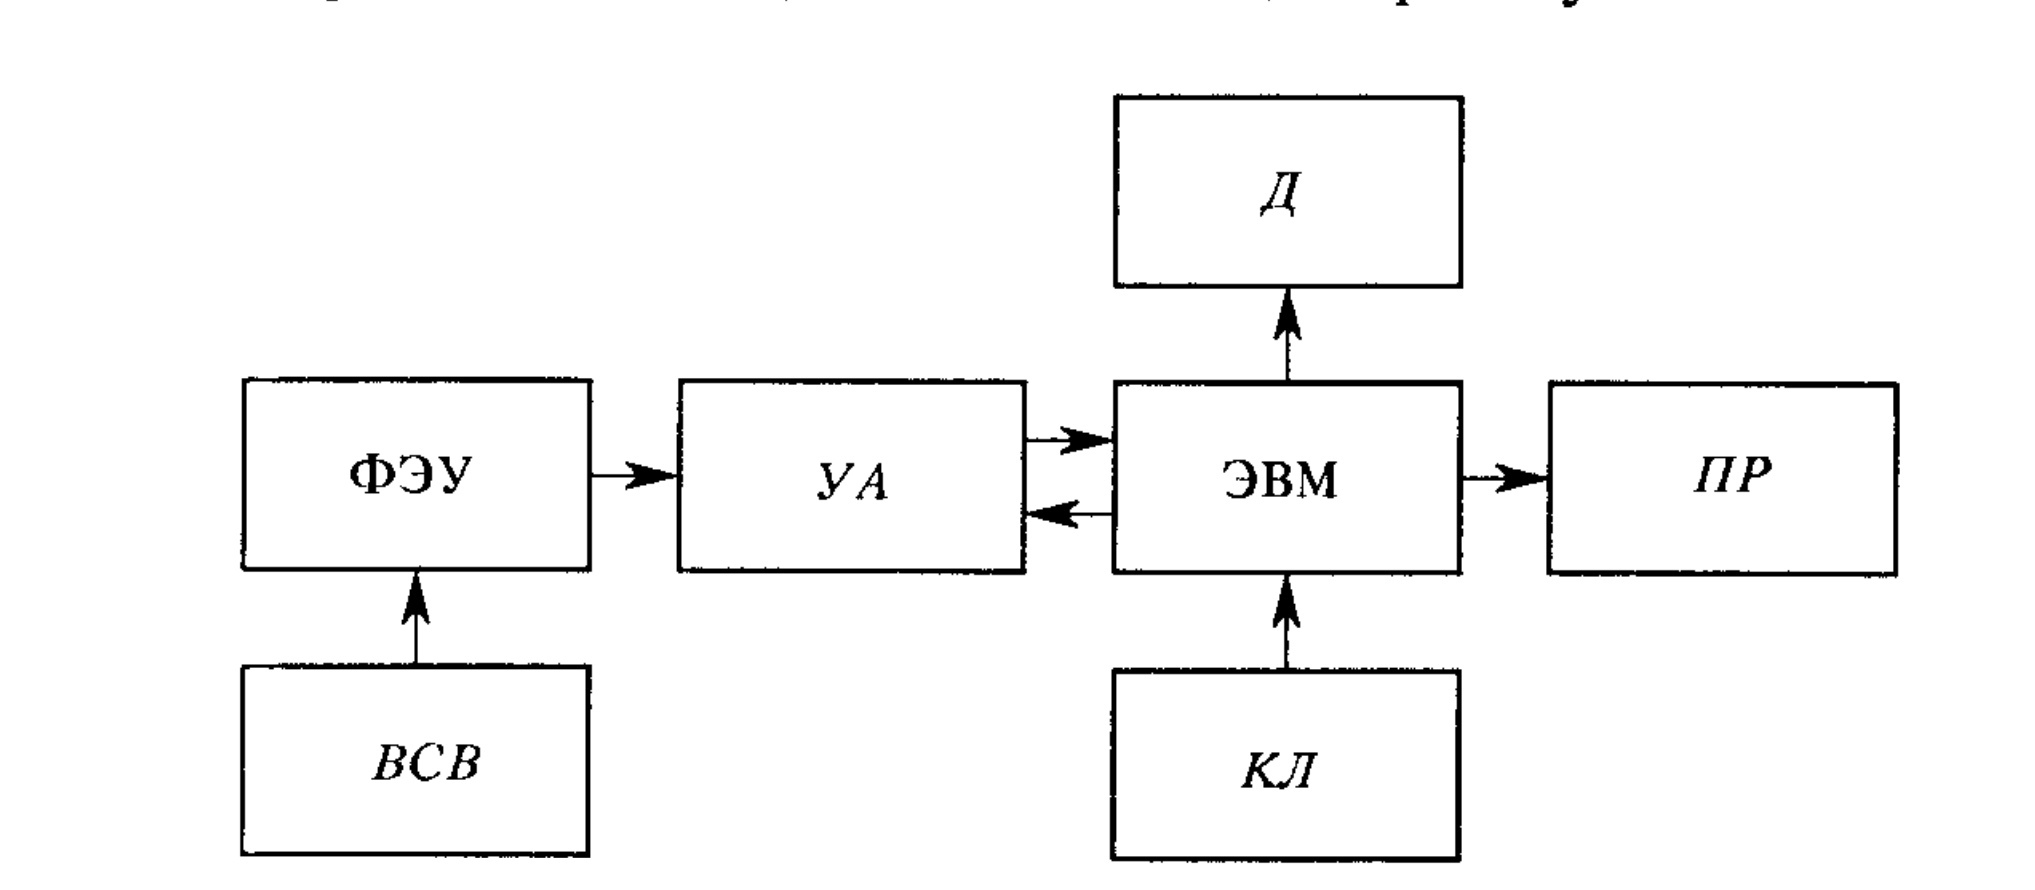
\includegraphics[width=1\textwidth]{izmerit.jpg}
    \caption{Измерительный комплекс}
    \label{fig:izm}
\end{figure}
Измерительный комплекс состоит из ФЭУ, питаемого от высоковольтного выпрямителя ВСВ, усилителя-анализатора УА, являющегося входным интерфейсом компьютера ЭВМ, управляемого с клавиатуры КЛ. Информация отображается на дисплее Д. При работе ФЭУ в спектрометрическом режиме величина выходного электрического импульса пропорциональна энергии регистрируемого $\gamma$-кванта. В итоге возникает распределение электрических испульсов, имеющее фотопик, положение вершины которого нас будет интересовать. Левее фотопика начинается непрерывный спектр комптоновских электронов, который сохраняется при любом угле рассеяния. Номер канала на распределении соответствует энергии регистрируемой частицы, точность его определения примерно $1\%$.

\section{Обработка результатов}
В таблице представлены измеренные данные. Точка для 20 градусов отсутствует, так как в процессе орбаботки выяснилось, что она измерена плохо.

\begin{table}[H]
	\centering
	\begin{tabular}{|c|c|c|c|c|c|c|c|c|c|c|c|}
	\hline
	\textbf{Угол, град} & 0   & 10  & 30  & 40  & 50  & 60  & 70  & 80  & 90  & 100 & 110 \\ \hline
	\textbf{Канал, N}   & 915 & 896 & 761 & 695 & 608 & 541 & 478 & 431 & 383 & 350 & 330 \\ \hline
	\end{tabular}
	\end{table}

По этим данным построим график зависимости $ 1 / N(\theta)$ от $1 - cos(\theta)$:
\begin{figure}[H]
    \centering
    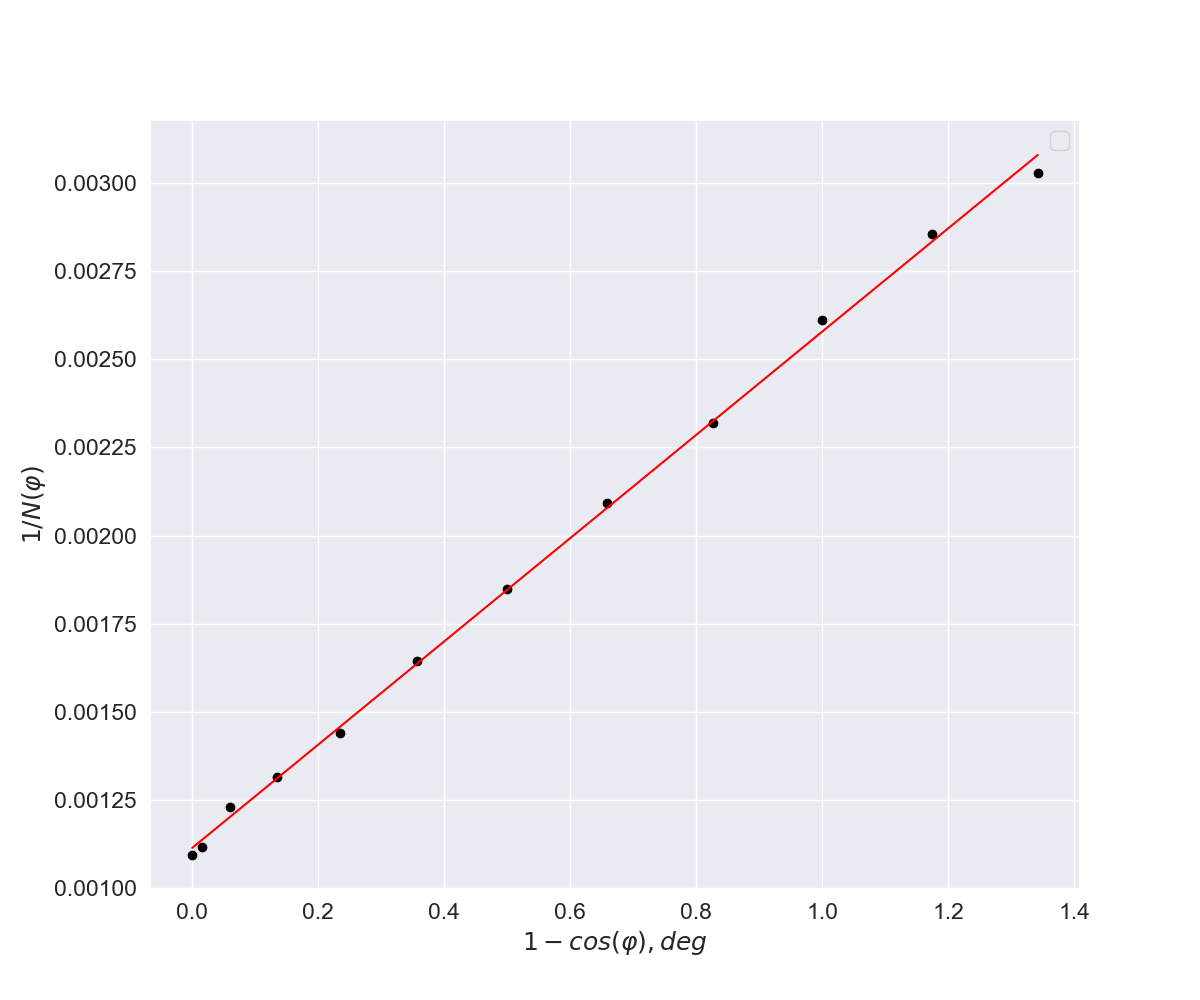
\includegraphics[width=1\textwidth]{plot.png}
    \caption{График по измеренным данным}
\end{figure}
Как видим, зависимость действительно линейная. На графике зеленым маркером отмечены интересующие нас точки для формулы (\ref{eq:main}):
\begin{equation*}
	N(0) = 911 \pm 24
\end{equation*}
\begin{equation*}
	N(90) = 385 \pm 14
\end{equation*}
Нам известна энергия $E_0$ = 662 кэВ. Тогда можем найти энергию искомую энергию покоя электрона:

\begin{equation}
	mc^2 = 485 \pm 30 \text{ кэВ}
\end{equation}
Истинная энергия покоя электрона 510 кэВ. Таким образом резульататы опыта совпали с истинным с точностью до погрешности.

\section{Выводы}

В работе было исследовано рассеяние гаммма-квантов, подтверждена теоретическая формула для распределения энергии в зависимости от угла рассеяния, посчитана энергия покоя электрона.

\end{document}